\documentclass{article}
\usepackage[utf8]{inputenc}
% Language setting
% Replace `english' with e.g. `spanish' to change the document language
\usepackage[english]{babel}
\usepackage[dvipsnames]{xcolor}

% Set page size and margins
% Replace `letterpaper' with `a4paper' for UK/EU standard size
\usepackage[a4paper,top=2cm,bottom=2cm,left=3cm,right=3cm,marginparwidth=1.75cm]{geometry}

\definecolor{commentsgreen}{HTML}{629755}
\definecolor{keyword}{HTML}{CC7832}
\definecolor{annot}{HTML}{BBB529}

% Useful packages
\usepackage{amsmath}
\usepackage{graphicx}
\usepackage{subfig}
\usepackage{comment}
\usepackage[colorlinks=true, allcolors=blue]{hyperref}
\usepackage{placeins}
\usepackage{float}
\usepackage{listings}
\usepackage[super]{nth}
\usepackage{hyperref}
\lstset{frame=tb,
  language=Java,
  aboveskip=5mm,
  belowskip=5mm,
  showstringspaces=false,
  columns=flexible,
  basicstyle={\small\ttfamily},
  numbers=none,
  numberstyle=\tiny\color{blue},
  keywordstyle=\color{keyword},
  commentstyle=\color{commentsgreen},
  stringstyle=\color{orange},
  breaklines=true,
  breakatwhitespace=true,
  moredelim=[s][\textcolor{annot}]{@}{\ },
  tabsize=3}

\title{Assignment 3: Refactoring the Design\\
of an Existing Project\\
\large Software Design and Modelling}

\author{Daniele Gasparini, Mattia Monari, Sergiu Gheorghita}
\date{\nth{28} November 2022}

\begin{document}

\maketitle

\section{Project Selection}
For the project selection each of us proposed some University projects we made in the previous semester whose design required a refactoring. We ended up selecting Mattia's project called "Sorting Algorithms Visualized Through Images"(SAVTI), because it will be used as starting point of his BSc thesis(he is an Erasmus student) and a deep refactoring is needed to make his life easier since as it is today the project presents some design anti-pattern that must be removed.

\section{Project Description}
SAVTI is a desktop application created for scholastic purpose for the \href{https://github.com/nbicocchi/ooprogramming}{OOP course from the Università degli Studi di Modena e Reggio Emilia.} It gives the possibility to randomize an image with a custom precision (which gets splitted in an array of tiles), choose a custom sorting algorithm and reorder it. This process will be encoded in a .mp4 video thanks to the \href{https://github.com/jcodec/jcodec}{jcodec} library, obtaining results similar to \href{https://youtu.be/4lyLJmZbQSA}{this}.
\newline 
\begin{figure} [h!]
    \centering
    \includegraphics[width=0.9 \linewidth]{seconda.jpg} 
    \caption{SAVTI GUI} 
    \label{GUI}
\end{figure}


\section{Refactoring Goals}
The refactoring we made had two main goals. The first one is to remove code smells inside the code, for this purpose we used SonarQube to detect part of the code whose design could be imporved. 
(addActionListeners in \textbf{savti.MainWindow.java} and \textbf{savti.MainWindow.java)}\\
The second one is to make the code more readable since the project presents complexity flaws in some classes which have very long methods. In this case we also added javadocs and tests to the project to make the maintenance of the code leaner.

\section{Refactoring examples}

\subsection{Fixing naming flaws}
By looking at the SonarQube report, the first thing we refactored was the naming of local variables, in this case we used a capital letter to represent a local variable so we decide to use a more readable variable for the RGB indexes instead.

\begin{comment}
\begin{figure}[!htb]
   \begin{minipage}{0.5\textwidth}
     \centering
     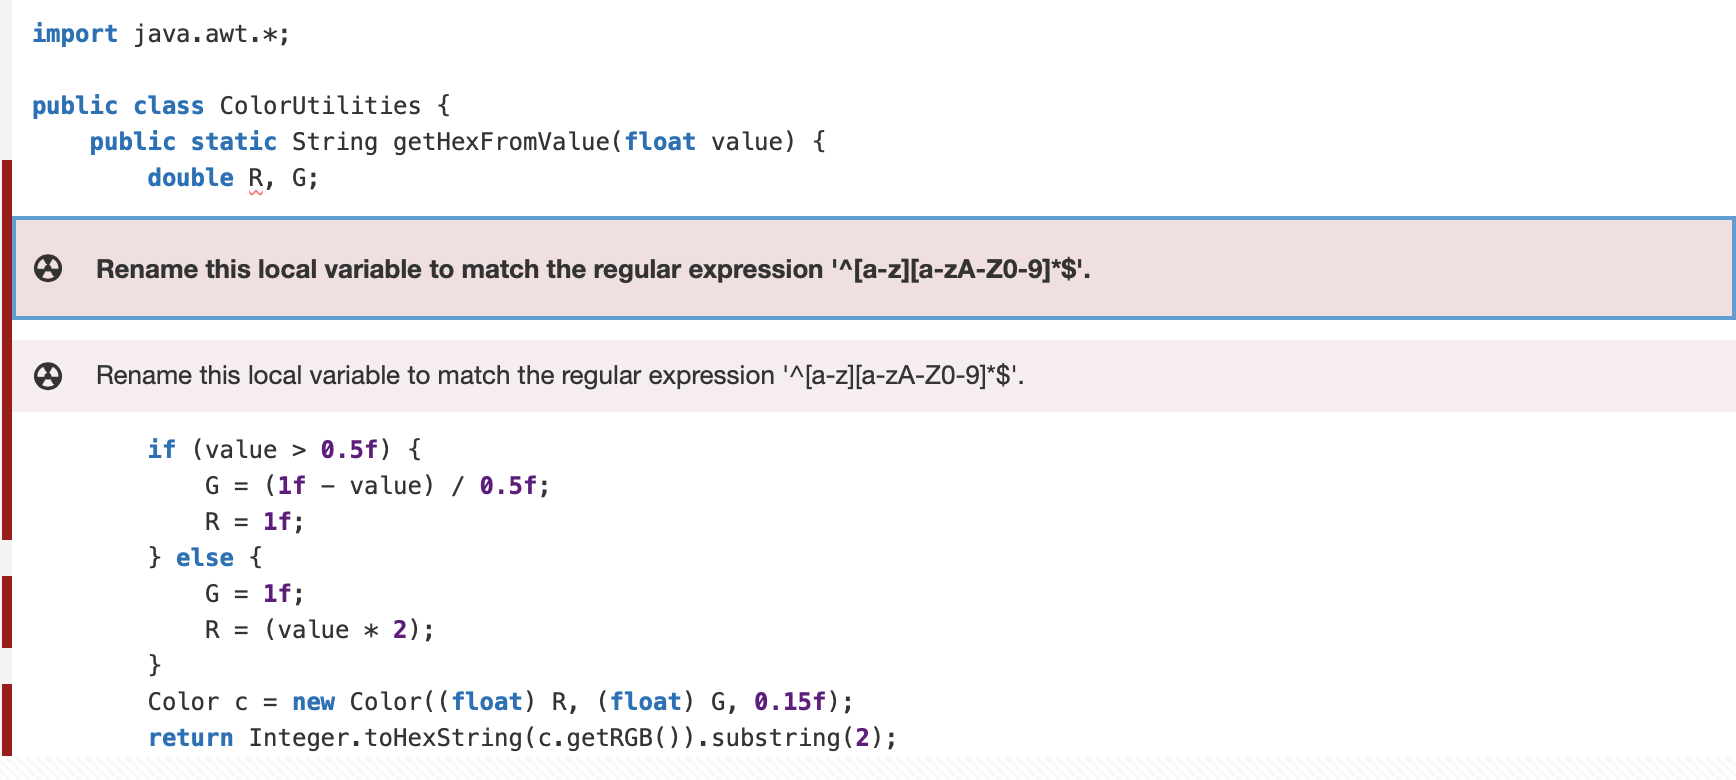
\includegraphics[width=1\linewidth]{Rename/Rename1.png}
   \end{minipage}\hfill
   \begin{minipage}{0.5\textwidth}
     \centering
     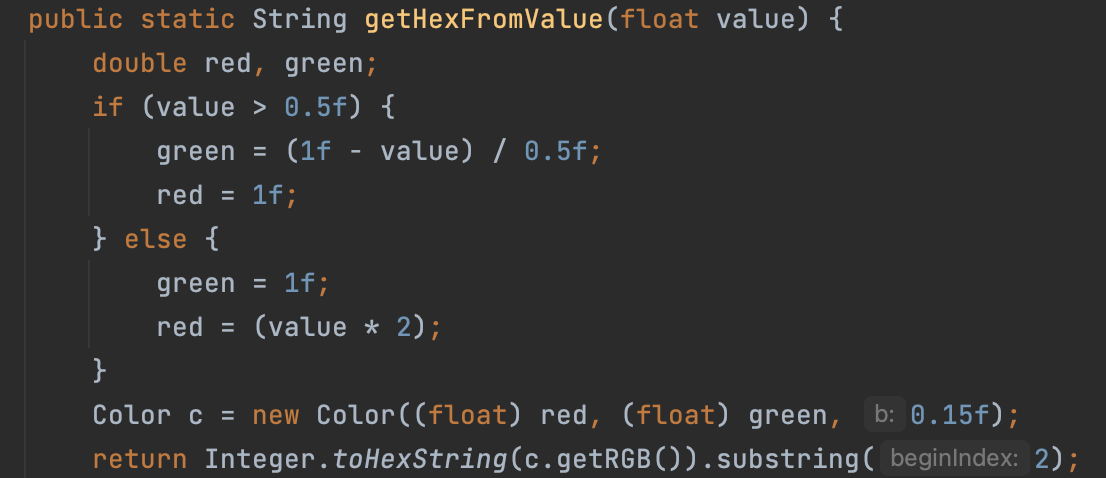
\includegraphics[width=1\linewidth]{Rename/Rename2.png}
   \end{minipage}
   \caption{Rename Local Variable and Method Parameters}\label{fig:Rename}
\end{figure}
\end{comment}
\begin{lstlisting}[caption={Fixing naming flaws},captionpos=b]
public static String getHexFromValue(float value) {
        double red, green; // before they were R and G
        if (value > 0.5f) {
            green = (1f - value) / 0.5f;
            red = 1f;
        } else {
            green = 1f;
            red = (value * 2);
        }
        Color c = new Color((float) red, (float) green, 0.15f);
        return Integer.toHexString(c.getRGB()).substring(2);
    }
\end{lstlisting}
\subsection{Collapsable If statement should be merged}
To solve this issue we merged the collapsable if statement to increase readability, for this reason we first merged the two condition as one by using the logical AND(&&).\\
Then, since the same sentence was used inside numerous classes(UserSettings, AdvancedSettings and MainWindow) we decided to reduce the coupling of the class and create a method called isOutputDirectory, inside the class UserSettings, whose purpose is to check that the output directory is not null and check that effectively it is a directory.
\begin{lstlisting}[language=Java,caption={Old Implementation},captionpos=b]
if (userSettings.getOutputDirectory() != null){
    if (userSettings.getOutputDirectory().isDirectory()){
\end{lstlisting}


\begin{lstlisting}[caption={New Implementation},captionpos=b]
public boolean isOutputDirectory() {
        return getOutputDirectory() != null && getOutputDirectory().isDirectory();
    }
    
\end{lstlisting}

\begin{lstlisting}[caption={Application of the new implementation},captionpos=b]
if (userSettings.isOutputDirectory())
            try {
                Desktop.getDesktop().open(userSettings.getOutputDirectory());
            } catch (IOException e) {
                ErrorUtilities.SWW();
            }
\end{lstlisting}

\begin{comment}

\begin{figure}[!htb]
     \centering
     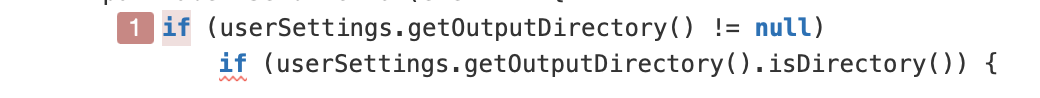
\includegraphics[width=1\linewidth]{CollapsableIF/CollapsableIF1.png}
     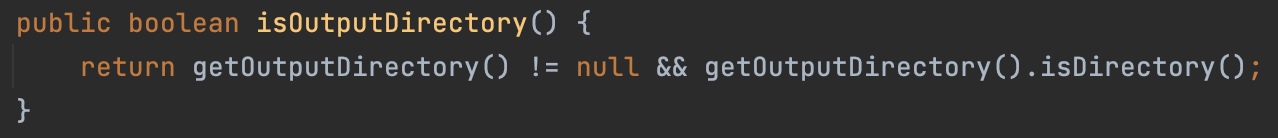
\includegraphics[width=1\linewidth]{CollapsableIF/CollapsableIF2.png}
     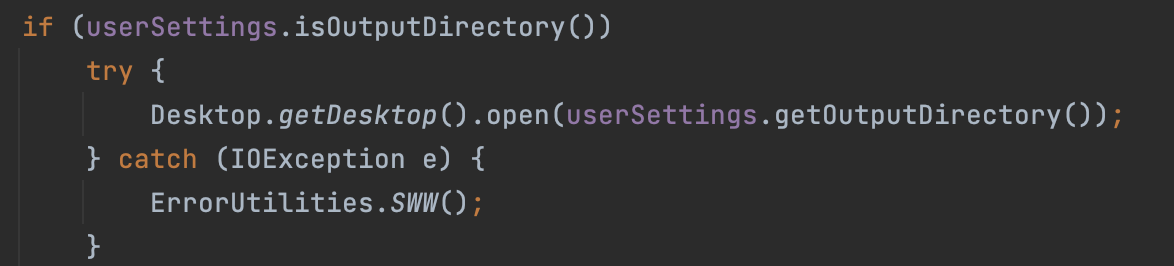
\includegraphics[width=1\linewidth]{CollapsableIF/CollapsableIF3.png}
     \caption{Collapsable If statement}
\end{figure}
\end{comment}

\subsection{Private fields only used as local variables in methods should become local variables}

In this case the private field is initiated with a builder, for this reason the tool thinks it is only used inside a method, but in reality it is initiated in the constructor by the method initComponents, this is already a form of refactoring, because instead of having a huge amount of parameters in the constructor, a method is used to initialize it.

\subsection{Documentation}
To increase readability and comprehension of the project we added java docs in that parts of the program whose structure was more complex and for all the classes we created to improve the design.\\
As an example we put below the documentation we implements for the LoadSongCommand, to do it we followed JavaDocs rules.

\begin{lstlisting}[caption={Adding JavaDocs},captionpos=b]

public class LoadSongCommand implements Command{
    MainWindow mainWindow;
    UserSettings userSettings ;
    /**
     * Constructor for LoadSongCommand class.
     * @param userSettings are the settings that will be changed after the load of the song
     */
    public LoadSongCommand(UserSettings userSettings, MainWindow mainWindow) {
        this.userSettings = userSettings;
        this.mainWindow = mainWindow;
    }
}
\end{lstlisting}
\begin{comment}
\begin{figure}[!htb]
    \centering
    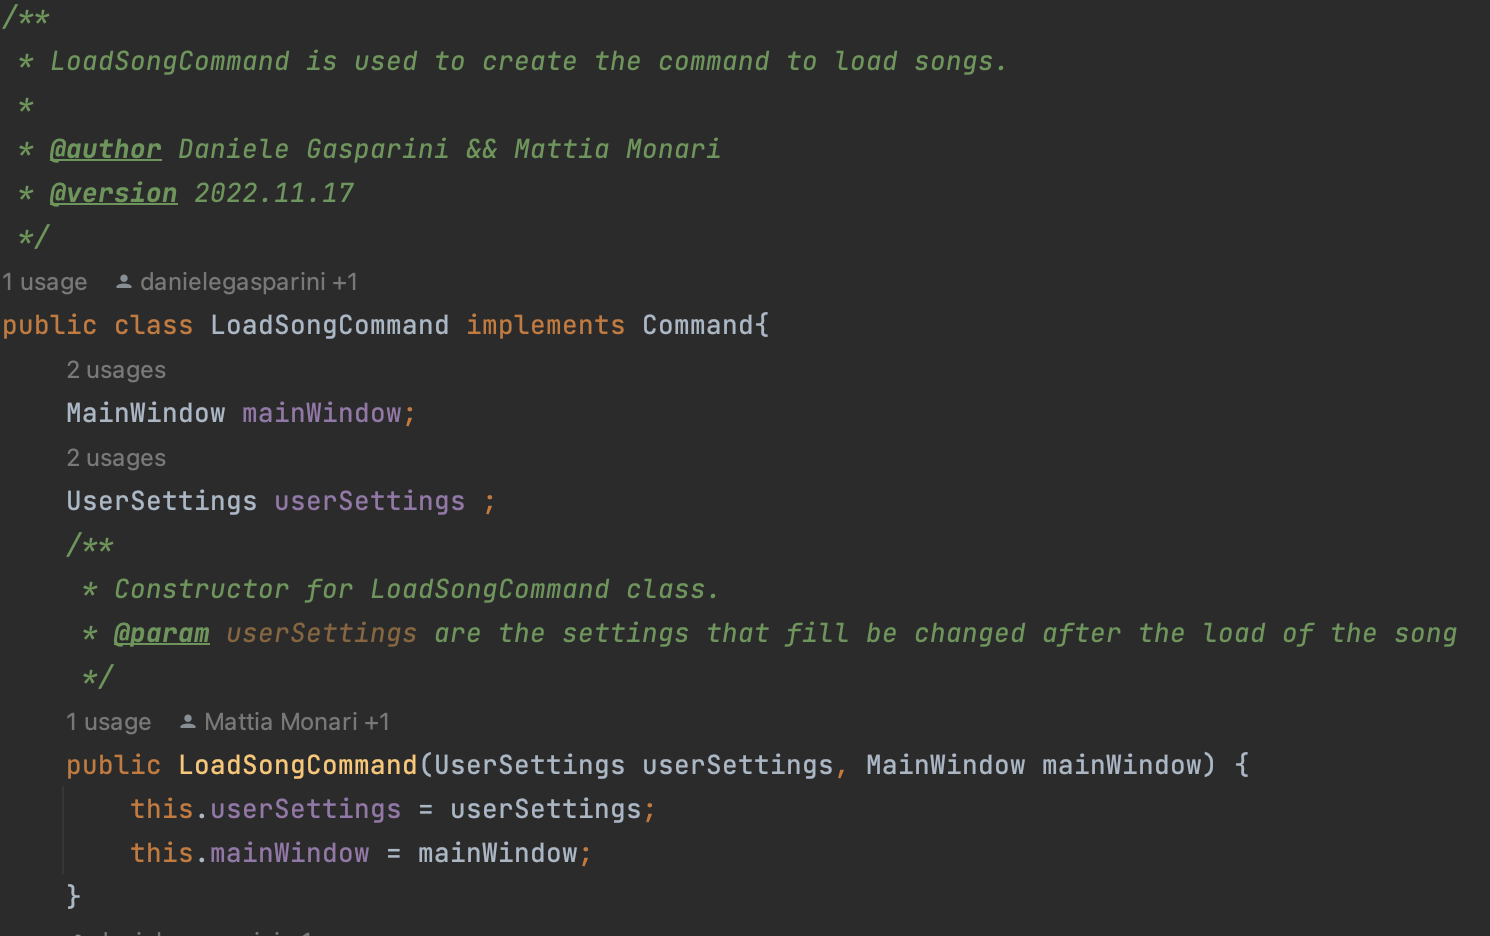
\includegraphics[width=1\linewidth]{Documentation/Documentation1.png}
    \caption{Caption}
    \label{fig:my_label}
\end{figure}

\end{comment}




\subsection{God classes and complexity flaws}
The majority of our work was to reduce the complexity of some God classes, which had a very high coupling and that presents some very long methods whose Cognitive complexity exceded the limit of 15 imposed by SonarQube.
We are talking about classes MainWindow and AdvancedSettings.\\
Our goal was to reach strong intra-class cohesion and loose inter-class coupling. 
For this reason in the case of MainWindow, whose purpose is to manage the GUI of the project, we made three distinct works.\\
First, by following the Single Responsibility Principle, we created custom UI classes which grouped togheter similar nodes; initially, \textbf{savti.MainWindow.java} class was managin each UI element by itself, now the subclasses we created are responsible for different parts of the UI. Here's the list of variables (annotated with the @FXML tag) in the \textbf{savti.MainWindow.java} class before and after the refactoring: 

\begin{minipage}{0.5 \textwidth}
\begin{lstlisting}[caption = {Variable before refactoring}]
    @FXML
    ImageView imageView;
    @FXML
    MenuItem imageLoaderItem;
    @FXML
    MenuItem songLoaderItem;
    @FXML
    MenuItem advSett;
    @FXML
    Button randomizeButton;
    @FXML
    Button sortingButton;
    @FXML
    Button cleanButton;
   //For each button
    
    
\end{lstlisting}
\end{minipage}
\begin{minipage}{0.5 \textwidth}
\begin{lstlisting}[caption = {Variables after refactoring}]
    @FXML
    ImageView imageView;
    
    @FXML
    Label headerText;
    
    @FXML
    ToggleSwitch darkMode;
    
    @FXML
    VBox menuVBox;
    
    MainVBox mainVBox;
    
    MainMenu mainMenu;
\end{lstlisting}  
\end{minipage}
\newpage
What we did was moving all those node which in the UI were togheter (see Figure \ref{GUI}) in a separate class, obtaining \textbf{savti.MainVBox.java and savti.MainMenu.java}. This classes had to be a UI node themselves, in order to display other elements. After encapsulating each field, we created the getters and replaced were necessary the usage of the nodes.

Then, we modified the method addEventListener, whose  purpose was to add a listener for each of the button inside the GUI. This method had a cognitive complexity of 55 and was composed by 257 lines of code, in pills it added a new event listener for each button by using lambda expression as shown in the snippet below.

\begin{lstlisting}[caption={Old Implementation},captionpos =b]
private void addEventListeners() {
        cleanButton.setOnAction(e -> {
            image.clearImage();
            imageView.setImage(null);
             deleteAllPreviousFiles(userSettings);
         });
\end{lstlisting}

The first modify we applied was to create a method for each EventListenr, so to reduce the complexity of the addEventListener method.

\begin{lstlisting}[caption={First modifies},captionpos =b]
private void cleanImageListener() {
         cleanButton.setOnAction(e -> {
             image.clearImage();
             imageView.setImage(null);
             deleteAllPreviousFiles(userSettings);
         });
     }
     
private void addEventListeners() {
         cleanImageListener();
         setAdvancedSettingsListener();
         loadImageListener();
         loadSongListener();
         setOutputPathListener();
         setDarkModeListener();
         randomShuffleListener();
         sortImageListener();
         burstModeToolTipListener();
         setBurstModeListener();
         clickToPathListener();
    }
\end{lstlisting}
Solved this smell we had to reduce the coupling of the class, for this reason we applied the Command pattern and the principle of separation of concerns, which usually results in breaking an app into layers.
We build an interface Command that was implemented by each concrete command, which represents a command to execute when a button is pressed.
Each concrete command is then called inside the addEventListeners method by a call on action.
Here is a snippet of the code implementation.
\begin{comment}
For doing this we followed this scheme.

\begin{figure}[!htb]
    \centering
    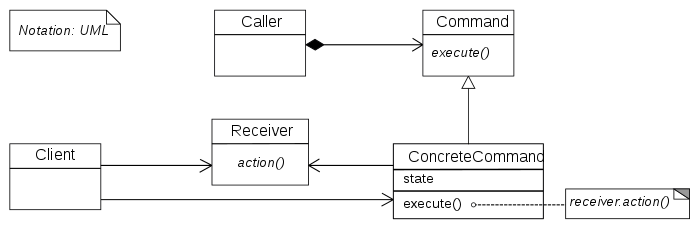
\includegraphics[width=1\linewidth]{700px-Command_pattern.svg.png}
    \caption{Command Pattern}
    \label{fig:my_label}
\end{figure}
\end{comment}


\begin{lstlisting}[caption={Command},captionpos=b]
public CleanImageCommand(TiledImage image, UserSettings userSettings, javafx.scene.image.ImageView imageView) {
        this.image = image;
        this.userSettings = userSettings;
        this.imageView = imageView;
    }
    @Override
    public void execute() {
        image.clearImage();
        imageView.setImage(null);}
\end{lstlisting}


\begin{lstlisting}[caption={Client},captionpos =b]
 private void addEventListeners() {
    mainVBox.getCleanButton().setOnAction(
                                e -> new CleanImageCommand(
                                    image, userSettings, imageView)
                                    .execute());
\end{lstlisting}
In this way we have also increased the cohesion, since we developed a set of classes responsible for the execution of the command of each button and we reduced the amount of work made by the god class \textbf{savti.MainWindow.java}.
The number of lines of the \textbf{savti.MainWindow.java} class were reduce from 520 up to 131: just the addEventListeners method itself were previously occupying 257 lines.
We used the same approach to improve the readability and to reduce the complexity of the class \textbf{savti.AdvancedSetting.java}. According to SonarQube the code still presents some method with high Cognitive Complexity, all these cases are methods of the sorting classes, we decided not to refactor it because they follow the standard sorting algorithms that are commonly used by developers community.
\\

\subsection{Method "clone" should not be overridden}
According to SunarQube report: "Many consider clone and Cloneable broken in Java, largely because the rules for overriding clone are tricky and difficult to get right; A copy constructor or copy factory should be used instead.". This rules is consider a blocker for a program, the highest level of error in SonarQube, so we decided to refactor the classes which was overriding the clone method and implement a copy factory method. Here's an example from \textbf{savti.Tile.java}:

    \begin{lstlisting}[caption={First clone implementation},captionpos =b]
    @Override
    public Tile clone() throws CloneNotSupportedException {
        Tile clone = (Tile) super.clone();
        clone.setX(this.x);
        clone.setY(this.y);
        clone.currentPosition = this.currentPosition;
        return clone;
    }
    \end{lstlisting}
    
    \begin{lstlisting}[caption={Clone Factory Method},captionpos =b]
     public Tile(Tile tile) {
        this.setX(tile.getX());
        this.setY(tile.getY());
        this.setCurrentPosition(tile.getCurrentPosition());
        this.initialPosition = tile.initialPosition;
        this.tile = tile.getTile();
    }

    public static Tile newInstance(Tile tile) {
        return new Tile(tile);
    }
\end{lstlisting}
\newpage
\subsection{Code clones}
The project presented numerous pieces of code that were textually very similar to other, in this case we used the extract method refactoring, as in the case of method writeFrame in class \textbf{savti.FileUtilities.java}.
In this case the class presents two methods with the same name, similar purpose but with different parameters. What we have done was to remove the duplicated parts of the code from the writeFrame method and create two sub methods that execute the cloned code.
In this case we had also to solve another problem because at first we called imageToFrameHeight method setFrameHeight, but this is a naming anti-pattern since we were calling an accessor method with a mutator naming standard(SET).\\
\begin{minipage}{0.5 \textwidth}
\begin{lstlisting}
    public static void writeFrame(AWTSequenceEncoder encoder, TiledImage image, UserSettings userSettings) {
         int width = (int) ( (image.getArray()[0].getWidth() * userSettings.getColsNumber()) % 2 == 0 ? image.getArray()[0].getWidth() * userSettings.getColsNumber() : image.getArray()[0].getWidth() * userSettings.getColsNumber() + 1);
         int heigth = (int) ( (image.getArray()[0].getHeight() * userSettings.getRowsNumber()) % 2 == 0 ? image.getArray()[0].getHeight() * userSettings.getRowsNumber() : image.getArray()[0].getHeight() * userSettings.getRowsNumber() + 1);
         BufferedImage finalImage = new BufferedImage(width, heigth, BufferedImage.TYPE_3BYTE_BGR);
         Graphics2D graphics2D = finalImage.createGraphics();
         .
         .
         .
         .
         .
         .
     }
\end{lstlisting}
\end{minipage}
\begin{minipage}{0.5 \textwidth}
\begin{lstlisting}
     public static void writeFrame(OutputHandler outputHandler, TiledImage image) {
        BufferedImage finalImage = buildFinalImage(image);
        Graphics2D graphics2D = finalImage.createGraphics();
        .
        .
        .
        }
        
    public static BufferedImage buildFinalImage(TiledImage image) {
        int width = imageToFrameWidth(image);
        int height = imageToFrameHeight(image);
        BufferedImage finalImage = new BufferedImage(width, height, BufferedImage.TYPE_3BYTE_BGR);
        return finalImage;
    }
    
    public static int imageToFrameHeight(TiledImage image) {
        if (image.getImage().getHeight() % 2 == 0) {
            return (int) image.getImage().getHeight();
        } else {
            return (int) image.getImage().getHeight() + 1;
        }
    }
\end{lstlisting}
\end{minipage}
\captionof{lstlisting}{Before and after refactoring of cloning code}


\section{Refactoring testing} 
Eventually, we decided to add also some tests to the application, since they were not present before. In order to that, we used the maven artifact of the \href{https://github.com/TestFX/TestFX}{TestFX} library. It provides a rich collection of matchers and assertions to verify expected states of JavaFX scene-graph nodes. \\
The test implemented were mainly done on the GUI aspects of the program, such as:

\begin{itemize}
    \item Checking labels of the nodes
    \item Checking colours of the nodes
    \item Checking if the listeners of some nodes were doing the correct tasks
\end{itemize}
In the future, Mattia is planning to add more tests to reach an higher code coverage.

\section{Difficulties}
During the process we didn't find many difficulties, in some cases the work required us only to modify some variables name or to move some lines of code. Nevertheless we had always to be careful not to change the behaviour of the program with our actions and since we had to develop tests from scratch at the beginning we did not have the certainty that what we were doing was correct.\\
Moreover, the developing of the command pattern to reduce the complexity of the addEventListener method has been the hardest part. This required us to first project the changes we had to make and understand how to adapt our code to the guidlines of the command pattern;
in this case working step by step ,as we documented in chapter 4.5, helped us because in this way we could check that we were not modifying the behaviour of the code while we were applying heavy edits. Looking at several examples of the pattern application and being inspired by other codes we developed in the past helped us to apply the correct edits to the SAVTI project.\\
Another hard part was to produce the test for the GUI, even if we used a pre compiled library we have to consider that different operating systems give different rights to the application, so a test that passed in Windows give us problems in MacOS.

\section{Conclusion}
If we look back to how was the project before the refactoring and how it is now we can state that we get it cleaner and more readable for a developer that has to work on it from scratch, by looking at the SonarQube reports before and after the refactoring a huge improvement of the project design can be seen, just consider that before we had 133 code smells and after only 36, most of them are TODOs that we left in the project for future updates and other are the long methods of the sorting algorithms we mentioned before.

Nevertheless numerous modifies can be added, first of all new tests must be added, because there are several branches of the test that are not covered yet.\\
Second, an ENUM class to store all the possible algorithms name can be added, in this way you increase compile-time checking and avoid errors from passing invalid constants.\\
Third, documentation must be improved, because there are several parts of the project which does not have documentation.
Improve documentation.

\end{document}
